\chapter{(Ana/mini)conda}
\section{简介}
\subsection{conda}
anaconde是Python的全家桶，包含了编辑器、解释器以及conda包管理工具，但是太占地方

miniconda是一个更小的包，\textcolor{YBXRed}{只}包含了解释器和conda包管理工具，编辑器需要自己安装。

\subsection{虚拟环境}
\textcolor{blue}{\textbf{虚拟环境}}是一个独立的Python环境(具备完整第三方依赖的python)，可以在不同的项目中使用不同的Python版本和包。
    
\section{安装}  
\subsection{安装anaconda}
\subsubsection{Linux安装}
参考\cite{Arch安装anaconda}
\begin{lstlisting}[style=demostyle,numbers=none]
#如果不喜欢一打开conda执行下面语句
conda config --set auto_activate_base false
\end{lstlisting}

\subsection{安装miniconda}
\subsubsection{Linux安装}
访问\href{https://docs.anaconda.com/free/miniconda/miniconda-install/}{官网}下载miniconda安装包，然后执行
\begin{lstlisting}[style=demostyle,numbers=none]
$> wget https://repo.anaconda.com/miniconda/Miniconda3-latest-Linux-x86_64.sh
wget https://mirrors.tuna.tsinghua.edu.cn/anaconda/miniconda/Miniconda3-py39_4.9.2-Linux-x86_64.sh
$> chmod +x Miniconda3-latest-Linux-x86_64.sh
$> ./Miniconda3-latest-Linux-x86_64.sh
Miniconda3 will now be installed into this location:
/home/tony/miniconda3

  - Press ENTER to confirm the location
  - Press CTRL-C to abort the installation
  - Or specify a different location below
[/home/tony/miniconda3] >>> /home/tony/.application/miniconda3

#如果不喜欢一打开conda执行下面语句
$> conda config --set auto_activate_base false
$> export PATH="/home/bxyang/opt/miniconda/bin:$PATH"
\end{lstlisting}

修改开头
\begin{lstlisting}[style=demostyle,numbers=none]
(/home/bxyang/.local/conda_env/lora) tony@gusu:~/Lora$ conda config --set env_prompt '({name})'
(/home/bxyang/.local/conda_env/lora) tony@gusu:~/Lora$ conda deactivate
(miniconda)tony@gusu:~/Lora$ conda activate lora
(lora)tony@gusu:~/Lora$
\end{lstlisting}

\subsubsection{Windows安装}
\label{sec:install_miniconda_windows}
访问\href{https://mirrors.tuna.tsinghua.edu.cn/anaconda/miniconda/}{清华大学镜像站}下载miniconda安装包，然后执行

\begin{figure}[htbp]
    \centering 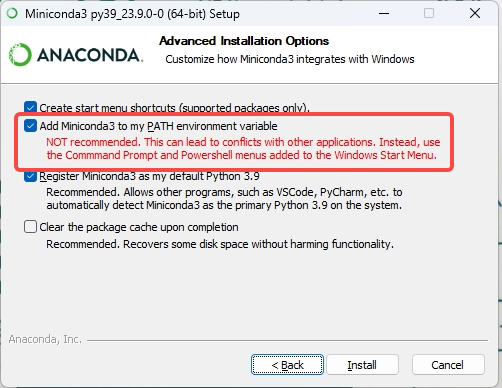
\includegraphics[width=.6\linewidth]{part/软件工程/环境搭建/虚拟环境/anaconda/pic/miniconda_windows环境变量.png}
      \caption{\label{fig:miniconda_windows环境变量}windows 安装miniconda配置环境变量}
\end{figure}

\reminder{\lefthand}{就算这步没有选择，可以安装以后手动配置环境变量，但是这样做会更麻烦一些。}

如图\ref{fig:miniconda_windows环境变量}所示，勾选上配置环境变量，然后点击下一步，然后点击安装，等待安装完成。

如果安装成功，可以在命令行中输入\codeinline{conda}，如果出现如图\ref{fig:conda安装成功}所示的结果，说明安装成功。
\begin{figure}[htbp]
    \centering 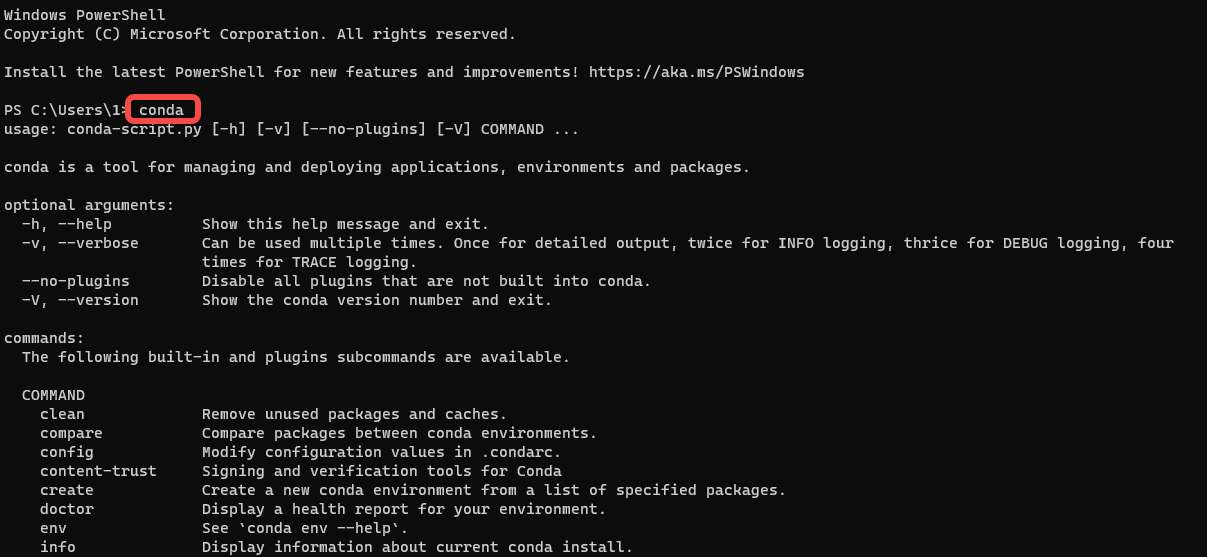
\includegraphics[width=.6\linewidth]{part/软件工程/环境搭建/虚拟环境/anaconda/pic/conda安装成功.png}
      \caption{\label{fig:conda安装成功}conda安装成功检验}
\end{figure}


\section{配置国内源}
\label{sec:use_conda_config}
各系统都可以通过修改用户目录下的 \codeinline{.condarc} 文件来使用 TUNA 镜像源
\subsection{linux}
\label{sec:use_conda_config_linux}
\begin{lstlisting}[style=demostyle,numbers=none]
$> vim ~/.condarc
channels:
  - defaults
show_channel_urls: true
default_channels:
  - https://mirrors.tuna.tsinghua.edu.cn/anaconda/pkgs/main
  - https://mirrors.tuna.tsinghua.edu.cn/anaconda/pkgs/r
  - https://mirrors.tuna.tsinghua.edu.cn/anaconda/pkgs/msys2
custom_channels:
  conda-forge: https://mirrors.tuna.tsinghua.edu.cn/anaconda/cloud
  msys2: https://mirrors.tuna.tsinghua.edu.cn/anaconda/cloud
  bioconda: https://mirrors.tuna.tsinghua.edu.cn/anaconda/cloud
  menpo: https://mirrors.tuna.tsinghua.edu.cn/anaconda/cloud
  pytorch: https://mirrors.tuna.tsinghua.edu.cn/anaconda/cloud
  pytorch-lts: https://mirrors.tuna.tsinghua.edu.cn/anaconda/cloud
  simpleitk: https://mirrors.tuna.tsinghua.edu.cn/anaconda/cloud
  deepmodeling: https://mirrors.tuna.tsinghua.edu.cn/anaconda/cloud/
 
$> conda info
\end{lstlisting}
\begin{figure}[htbp]
    \centering 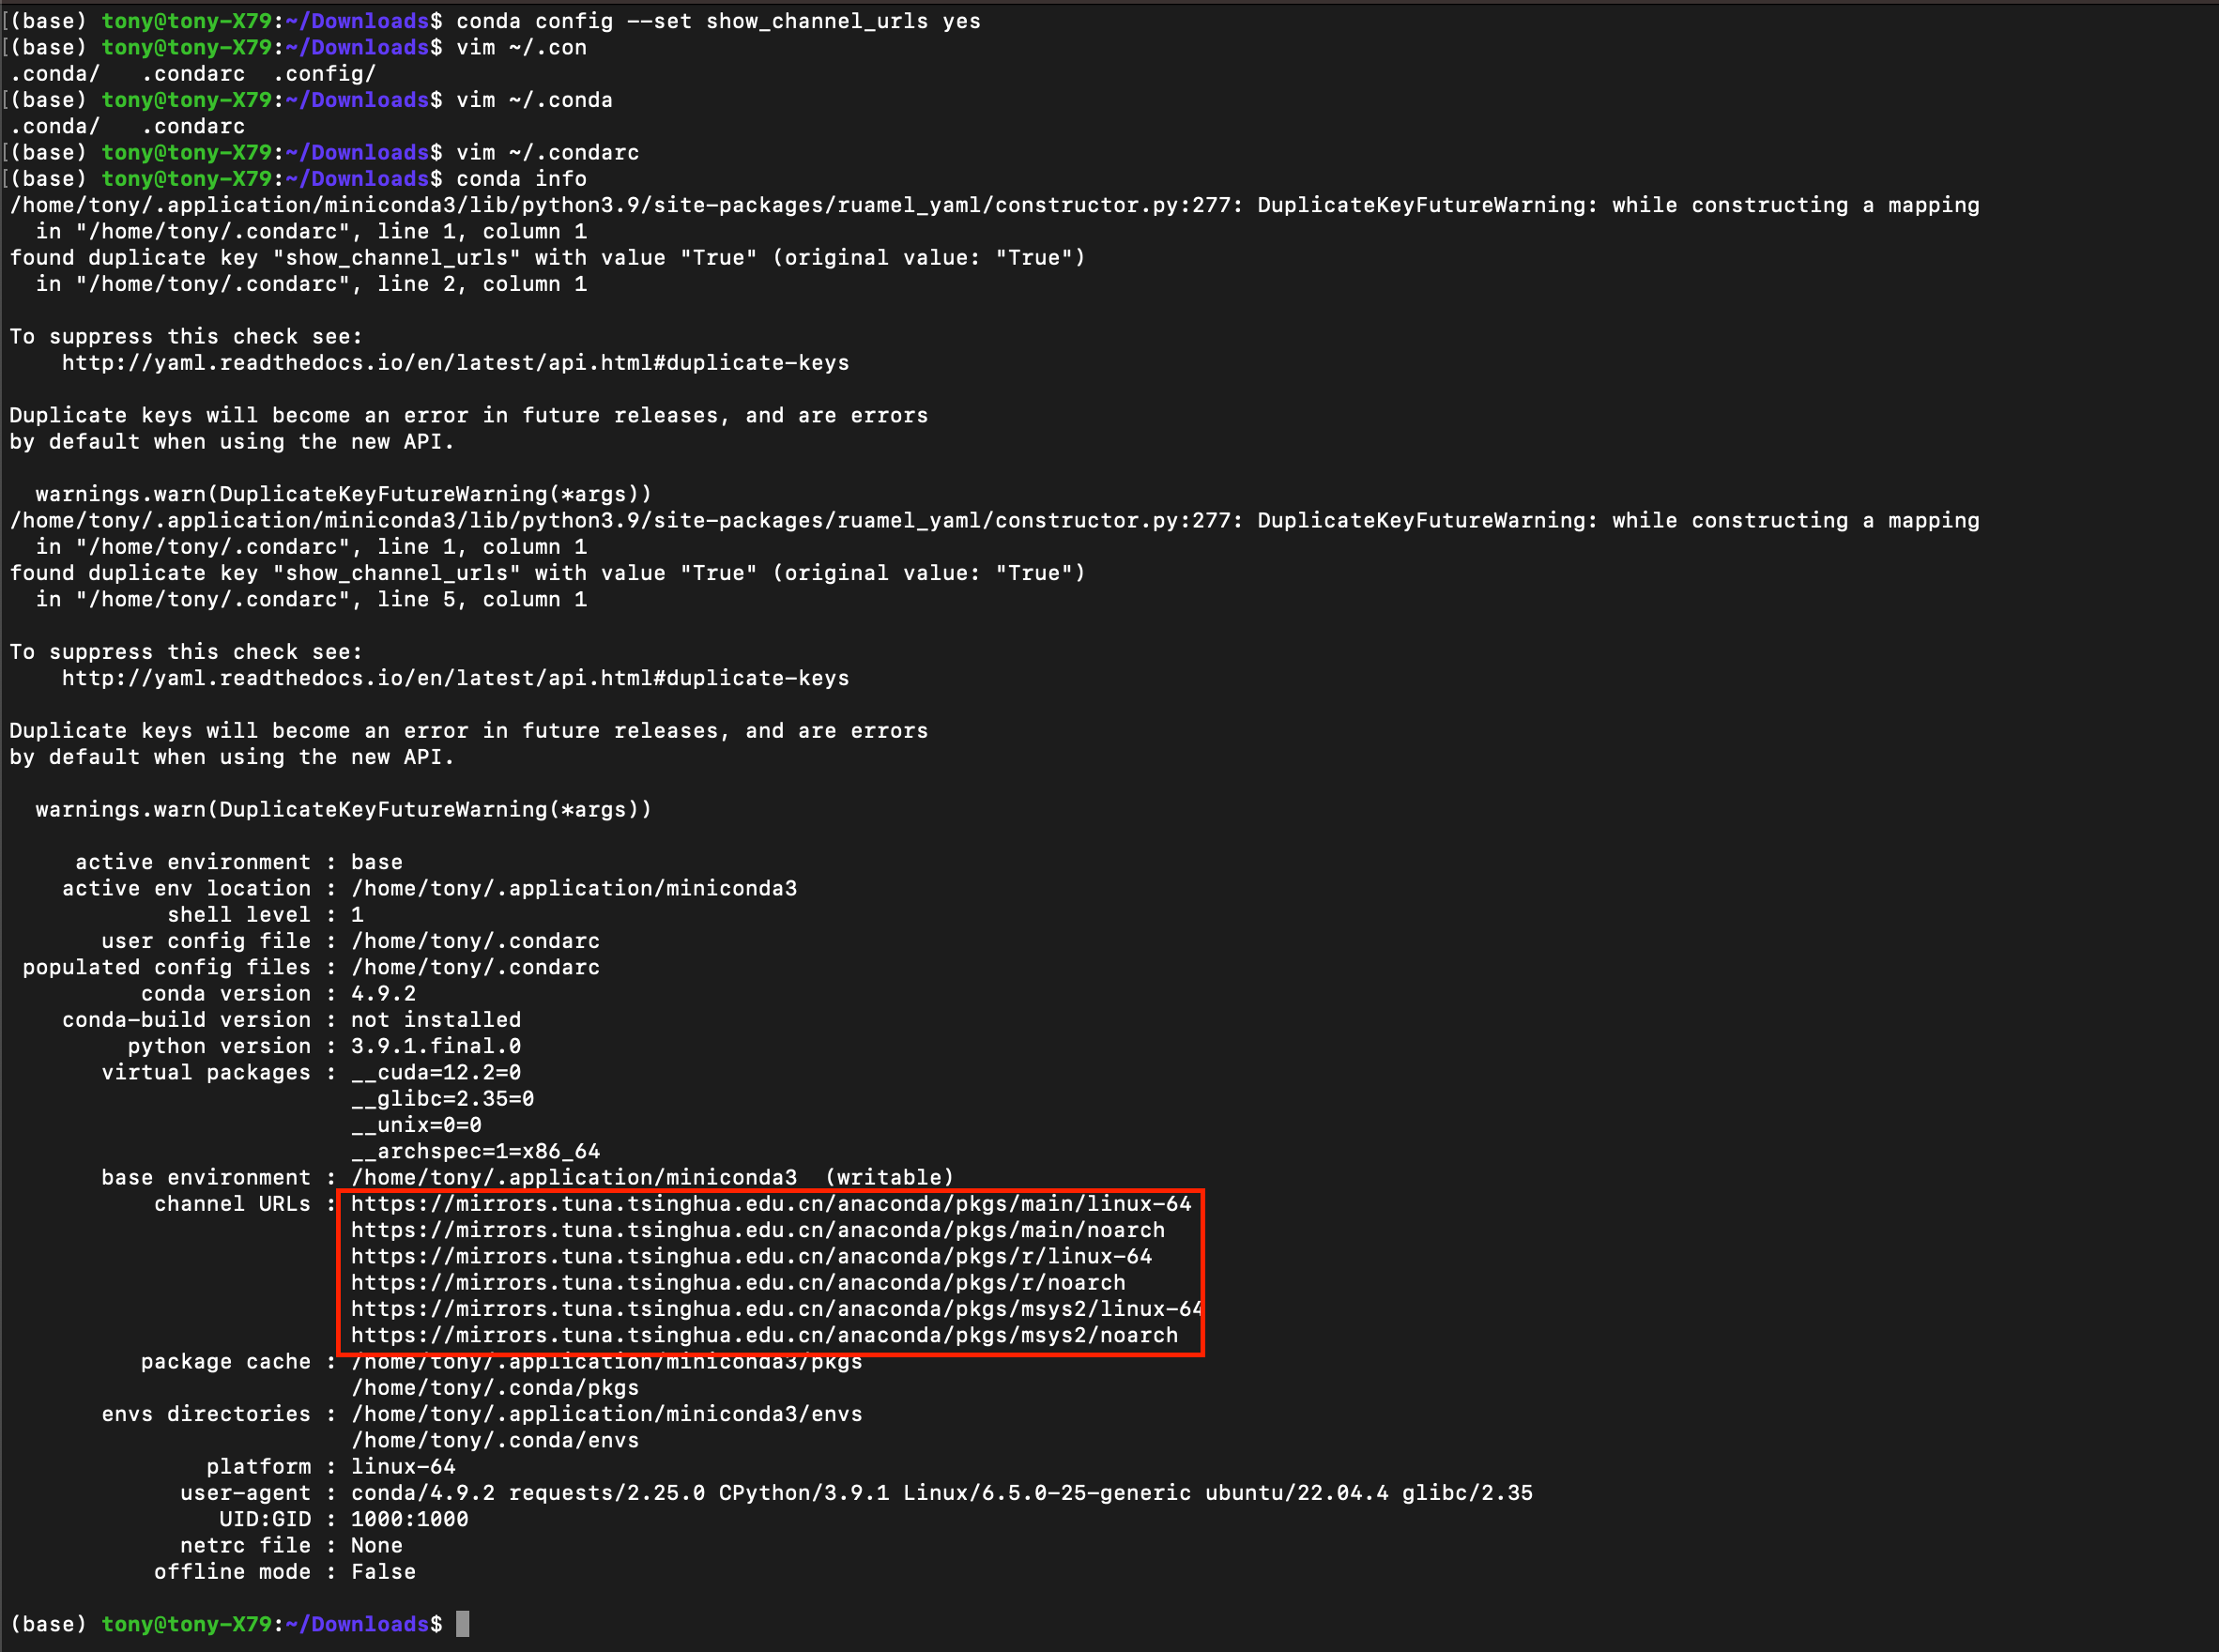
\includegraphics[width=.6\linewidth]{part/软件工程/环境搭建/虚拟环境/anaconda/pic/linux_conda使用终端配置国内源.png}
      \caption{\label{fig:linux_conda使用终端配置国内源}conda使用终端配置国内源}
\end{figure}

\subsection{windows}
\subsubsection{手动配置}
Windows 用户无法直接创建名为 \codeinline{.condarc} 的文件，可先执行 

\begin{lstlisting}[style=demostyle,numbers=none]
conda config --set show_channel_urls yes 
\end{lstlisting}
生成该文件之后再修改。
\begin{lstlisting}[style=demostyle,numbers=none]
show_channel_urls: true
channels:
  - defaults
default_channels:
  - https://mirrors.tuna.tsinghua.edu.cn/anaconda/pkgs/main
  - https://mirrors.tuna.tsinghua.edu.cn/anaconda/pkgs/r
  - https://mirrors.tuna.tsinghua.edu.cn/anaconda/pkgs/msys2
custom_channels:
  conda-forge: https://mirrors.tuna.tsinghua.edu.cn/anaconda/cloud
  msys2: https://mirrors.tuna.tsinghua.edu.cn/anaconda/cloud
  bioconda: https://mirrors.tuna.tsinghua.edu.cn/anaconda/cloud
  menpo: https://mirrors.tuna.tsinghua.edu.cn/anaconda/cloud
  pytorch: https://mirrors.tuna.tsinghua.edu.cn/anaconda/cloud
  pytorch-lts: https://mirrors.tuna.tsinghua.edu.cn/anaconda/cloud
  simpleitk: https://mirrors.tuna.tsinghua.edu.cn/anaconda/cloud
  deepmodeling: https://mirrors.tuna.tsinghua.edu.cn/anaconda/cloud/
\end{lstlisting}
\begin{figure}[htbp]
    \centering 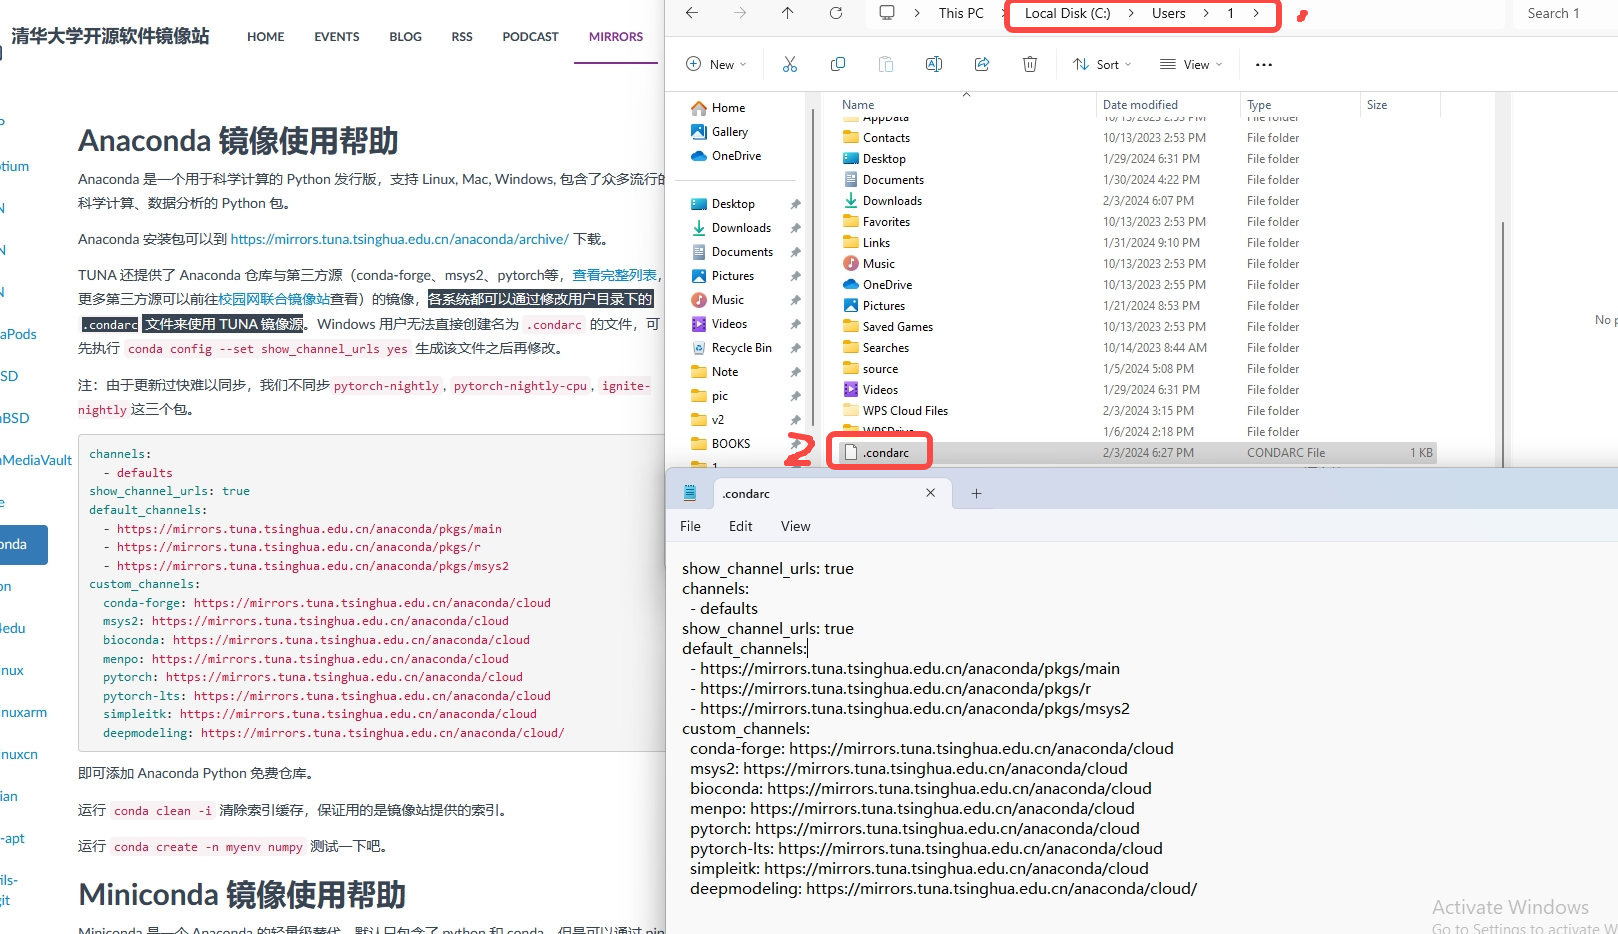
\includegraphics[width=.6\linewidth]{part/软件工程/环境搭建/虚拟环境/anaconda/pic/windows_conda使用配置文件配置国内源.png}
      \caption{\label{fig:windows_conda使用配置文件配置国内源}conda使用配置文件配置国内源}
\end{figure}

\subsubsection{命令行配置}
\label{sec:use_conda_config_windows_cmd}
如果嫌麻烦，可以直接在命令行中输入
\begin{lstlisting}[style=demostyle,numbers=none]
# 配置中科大源    
conda config --add channels https://mirrors.ustc.edu.cn/anaconda/pkgs/main/
conda config --add channels https://mirrors.ustc.edu.cn/anaconda/pkgs/free/
conda config --add channels https://mirrors.ustc.edu.cn/anaconda/cloud/conda-forge/
conda config --add channels https://mirrors.ustc.edu.cn/anaconda/cloud/msys2/
conda config --add channels https://mirrors.ustc.edu.cn/anaconda/cloud/bioconda/
conda config --add channels https://mirrors.ustc.edu.cn/anaconda/cloud/menpo/
conda config --add channels https://mirrors.ustc.edu.cn/anaconda/cloud/
# 阿里镜像源
conda config --add channels https://mirrors.aliyun.com/pypi/simple/
# 清华镜像源
conda config --add channels https://mirrors.tuna.tsinghua.edu.cn/anaconda/pkgs/main
conda config --add channels https://mirrors.tuna.tsinghua.edu.cn/anaconda/pkgs/r
conda config --add channels https://mirrors.tuna.tsinghua.edu.cn/anaconda/pkgs/msys2
# 清除索引缓存，保证用的是镜像站提供的索引
conda clean -i
# 显示检索路径，每次安装包时会将包源路径显示出来
conda config --set show_channel_urls yes
conda config --set always_yes True
# 显示所有镜像通道路径命令
conda config --show channels
# conda在指定环境下安装包
conda install -n machine_algorithm matplotlib
\end{lstlisting}    
\begin{figure}[htbp]
    \centering 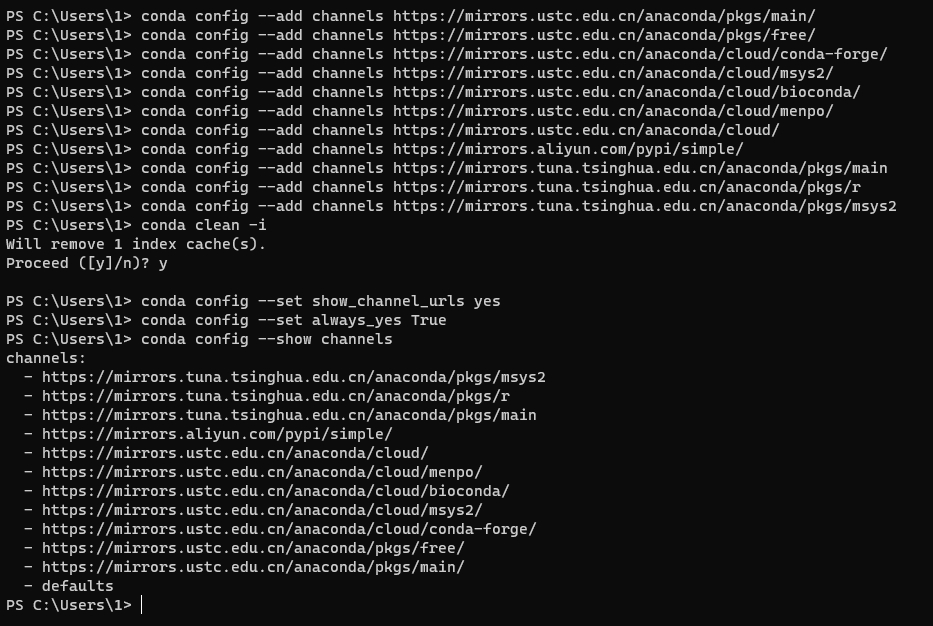
\includegraphics[width=.6\linewidth]{part/软件工程/环境搭建/虚拟环境/anaconda/pic/windows_conda使用终端配置国内源.png}
      \caption{\label{fig:windows_conda使用终端配置国内源}conda使用终端配置国内源}
\end{figure}

\subsubsection{移除镜像}
\label{sec:use_conda_config_windows_remove}
如果想要移除镜像，可以在命令行中输入
\begin{lstlisting}[style=demostyle,numbers=none]
conda config --remove channels 源名称或链接 
\end{lstlisting}    

\subsubsection{验证}
\label{sec:use_conda_config_windows_verify}
验证是否配置成功，可以在命令行中输入
\begin{lstlisting}[style=demostyle,numbers=none]
conda config --show-sources
# 或
conda info
\end{lstlisting}
如果出现如图\ref{fig:windows_conda使用终端配置国内源}所示的结果，说明配置成功。

\section{虚拟环境}
像Conda这样的包管理工具，管理的是\textcolor{YBXPurple}{虚拟环境}
\subsection{修改默认虚拟环境路径}
\begin{figure}[htbp]
    \centering 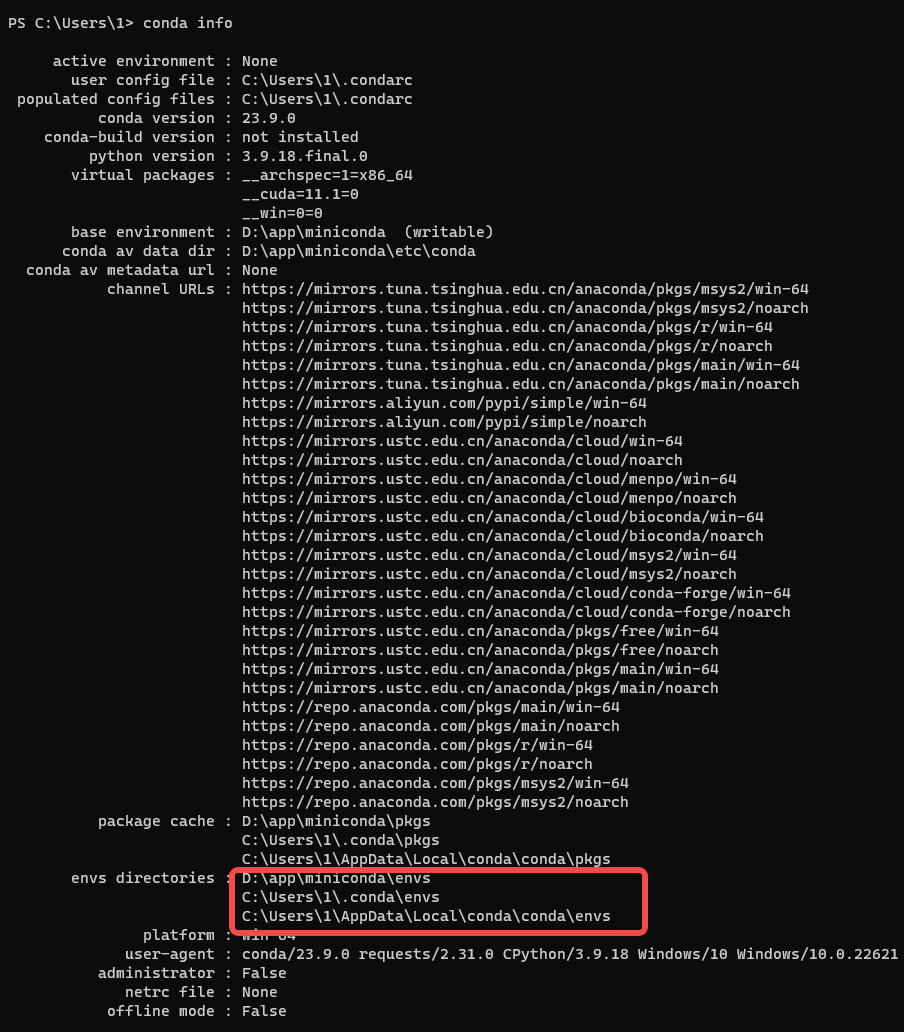
\includegraphics[width=.6\linewidth]{part/软件工程/环境搭建/虚拟环境/anaconda/pic/默认虚拟环境的默认路径.png}
      \caption{\label{fig:默认虚拟环境的默认路径}默认虚拟环境的默认路径}
\end{figure}

\subsubsection{Linux}
\begin{lstlisting}[style=demostyle,numbers=none]
$> mkdir  -p /home/tony/.local/conda_env # Linux
$> cat ~/.condarc
channels:
  - defaults
show_channel_urls: true
default_channels:
  - https://mirrors.tuna.tsinghua.edu.cn/anaconda/pkgs/main
  - https://mirrors.tuna.tsinghua.edu.cn/anaconda/pkgs/r
  - https://mirrors.tuna.tsinghua.edu.cn/anaconda/pkgs/msys2
custom_channels:
  conda-forge: https://mirrors.tuna.tsinghua.edu.cn/anaconda/cloud
  msys2: https://mirrors.tuna.tsinghua.edu.cn/anaconda/cloud
  bioconda: https://mirrors.tuna.tsinghua.edu.cn/anaconda/cloud
  menpo: https://mirrors.tuna.tsinghua.edu.cn/anaconda/cloud
  pytorch: https://mirrors.tuna.tsinghua.edu.cn/anaconda/cloud
  pytorch-lts: https://mirrors.tuna.tsinghua.edu.cn/anaconda/cloud
  simpleitk: https://mirrors.tuna.tsinghua.edu.cn/anaconda/cloud
  deepmodeling: https://mirrors.tuna.tsinghua.edu.cn/anaconda/cloud/

envs_dirs:
 - /home/tony/.local/conda_env
\end{lstlisting}  


\subsubsection{Windows}
在\codeinline{C:$\backslash$Users$\backslash$username$\backslash$.condarc}文件中添加如图\ref{fig:改变conda虚拟环境的默认路径}所示的内容，然后在命令行中输入

\begin{figure}[htbp]
    \centering 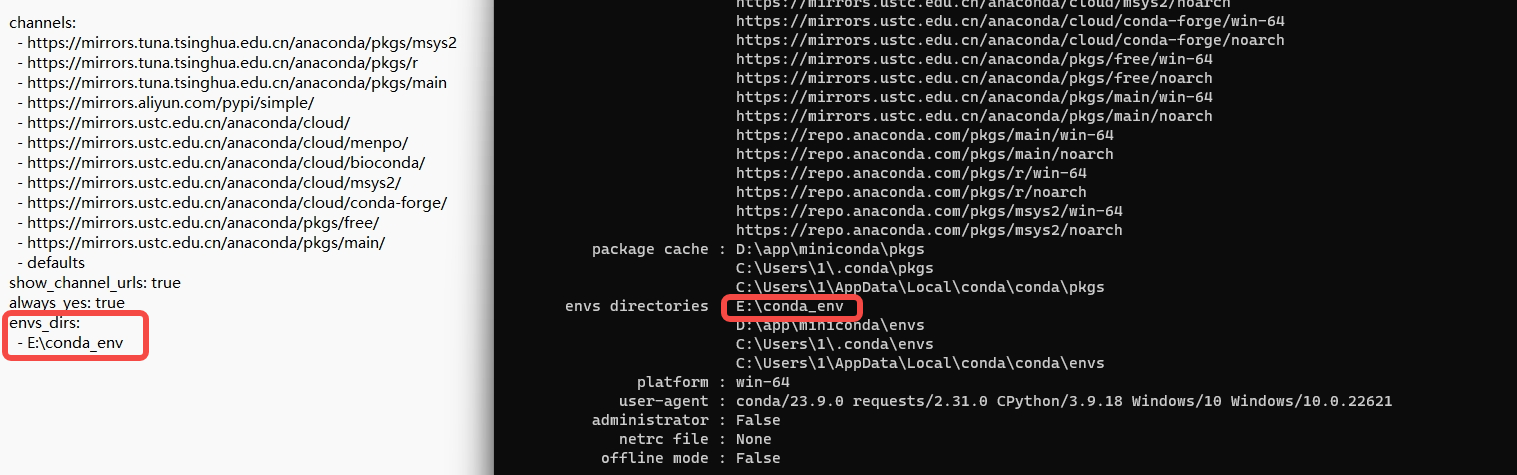
\includegraphics[width=.6\linewidth]{part/软件工程/环境搭建/虚拟环境/anaconda/pic/改变conda虚拟环境的默认路径.png}
      \caption{\label{fig:改变conda虚拟环境的默认路径}改变conda虚拟环境的默认路径}
\end{figure}


\subsection{创建虚拟环境}
\begin{lstlisting}[style=demostyle,numbers=none]
# 创建一个名为myenv的虚拟环境，指定Python版本是3.8，安装目录为E:\conda_env
conda create --name myenv python=3.9 -p E:\conda_env
\end{lstlisting}
\begin{figure}[htbp]
    \centering 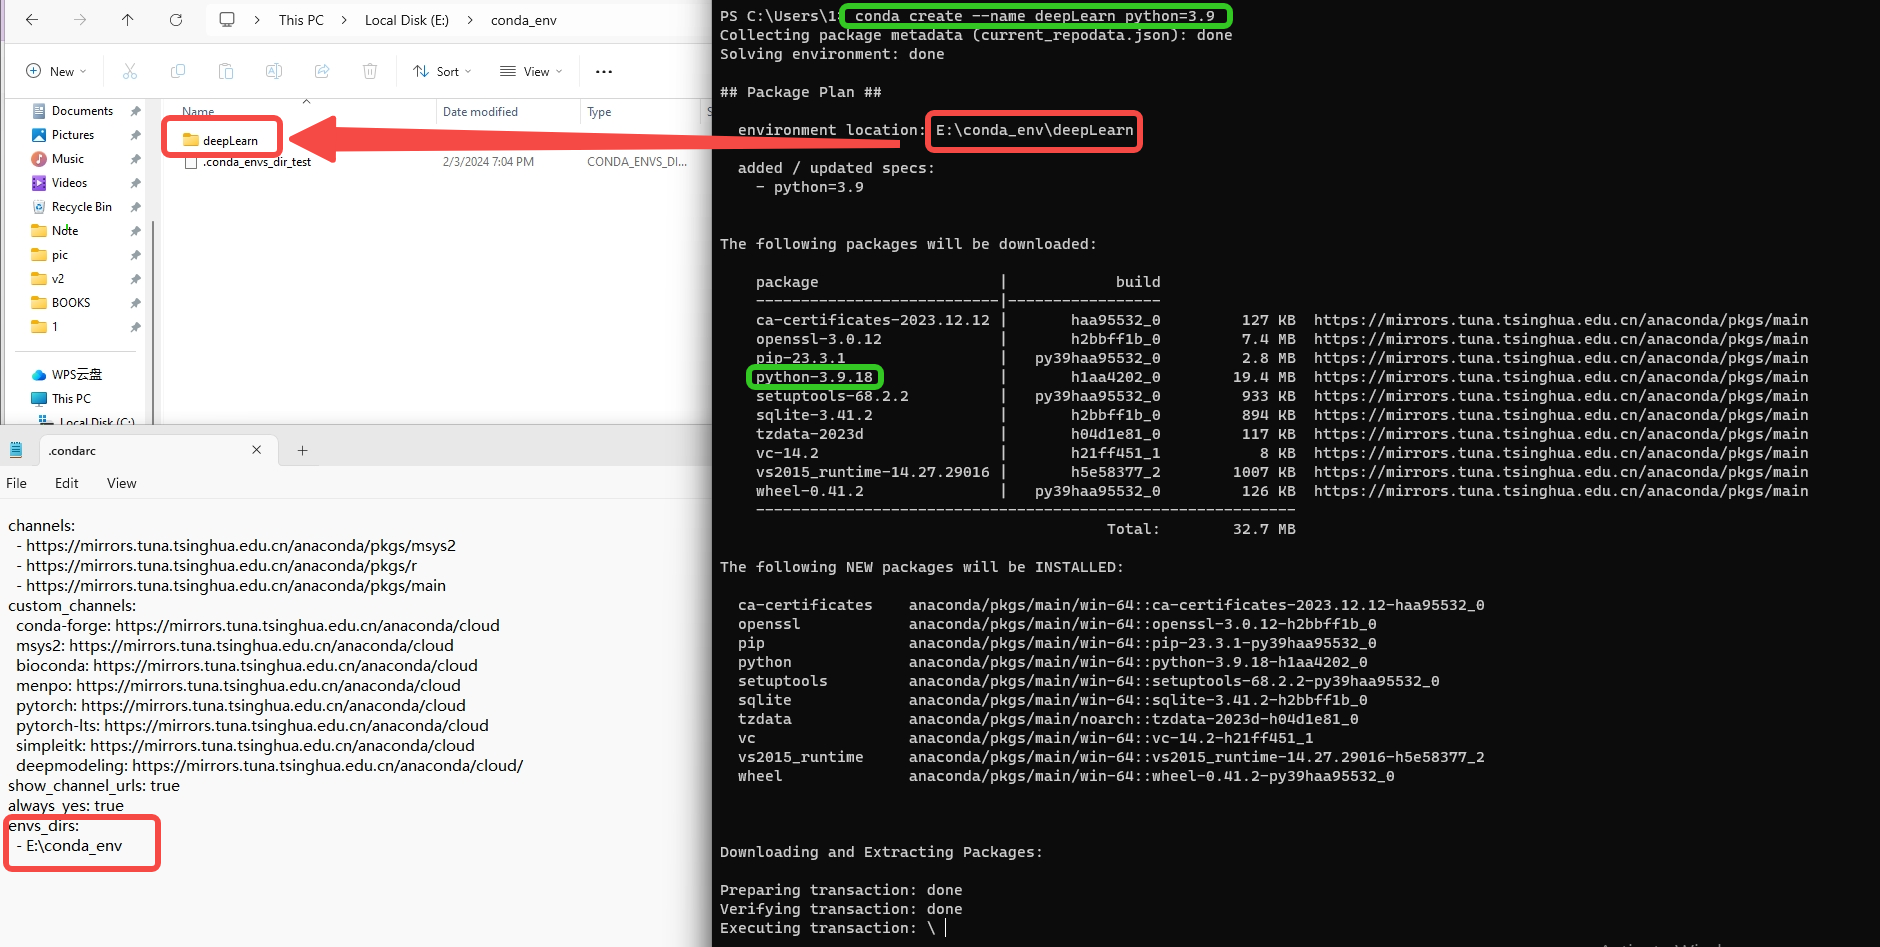
\includegraphics[width=.6\linewidth]{part/软件工程/环境搭建/虚拟环境/anaconda/pic/conda创建虚拟环境.png}
      \caption{\label{fig:conda创建虚拟环境}conda创建虚拟环境}
\end{figure}

\subsection{查看虚拟环境}
\label{subsubsec:use_conda_create_env_list}
\begin{lstlisting}[style=demostyle,numbers=none]
# 查看所有虚拟环境
conda info --envs
\end{lstlisting}
\begin{figure}[htbp]
    \centering 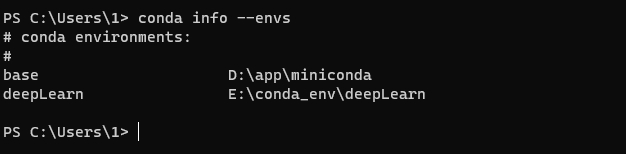
\includegraphics[width=.6\linewidth]{part/软件工程/环境搭建/虚拟环境/anaconda/pic/查看虚拟环境.png}
      \caption{\label{fig:查看虚拟环境}查看虚拟环境}
\end{figure}

\subsection{激活虚拟环境}
\begin{lstlisting}[style=demostyle,numbers=none]
# 激活虚拟环境
conda activate <env_name>
# 退出虚拟环境
conda deactivate
\end{lstlisting}

\subsection{删除虚拟环境}
在删除虚拟环境之前，需要先退出虚拟环境

\begin{lstlisting}[style=demostyle,numbers=none]
# 删除虚拟环境
conda remove --name <env_name> --all
\end{lstlisting}

\subsection{虚拟环境重新命名}
\begin{lstlisting}[style=demostyle,numbers=none]
# 重新命名虚拟环境
conda create --name new_name --clone old_name
\end{lstlisting}

\section{包管理}
\subsection{查询包}
\begin{lstlisting}[style=demostyle,numbers=none]
# 查询包
conda search <package_name>

# 安装指定版本的包
conda install <package_name>=<version>
\end{lstlisting}


\subsection{安装包}
\subsubsection{在线安装}
\subsubsubsection{conda安装}
conda安装包会自动安装相关依赖的包
\begin{lstlisting}[style=demostyle,numbers=none]
conda install pytorch torchvision torchaudio pytorch-cuda=11.8 -c pytorch -c nvidia
# -c 标志指定了要从哪个频道（channel）安装软件包。
# 频道是一组预先构建的二进制软件包的存储库，可以从中获取 Python 包和其他依赖项。频道可以位于 Anaconda 或第三方存储库中。
# 在使用 -c 标志时，可以在其后指定要使用的频道名称或 URL。
\end{lstlisting}
\begin{figure}[htbp]
    \centering 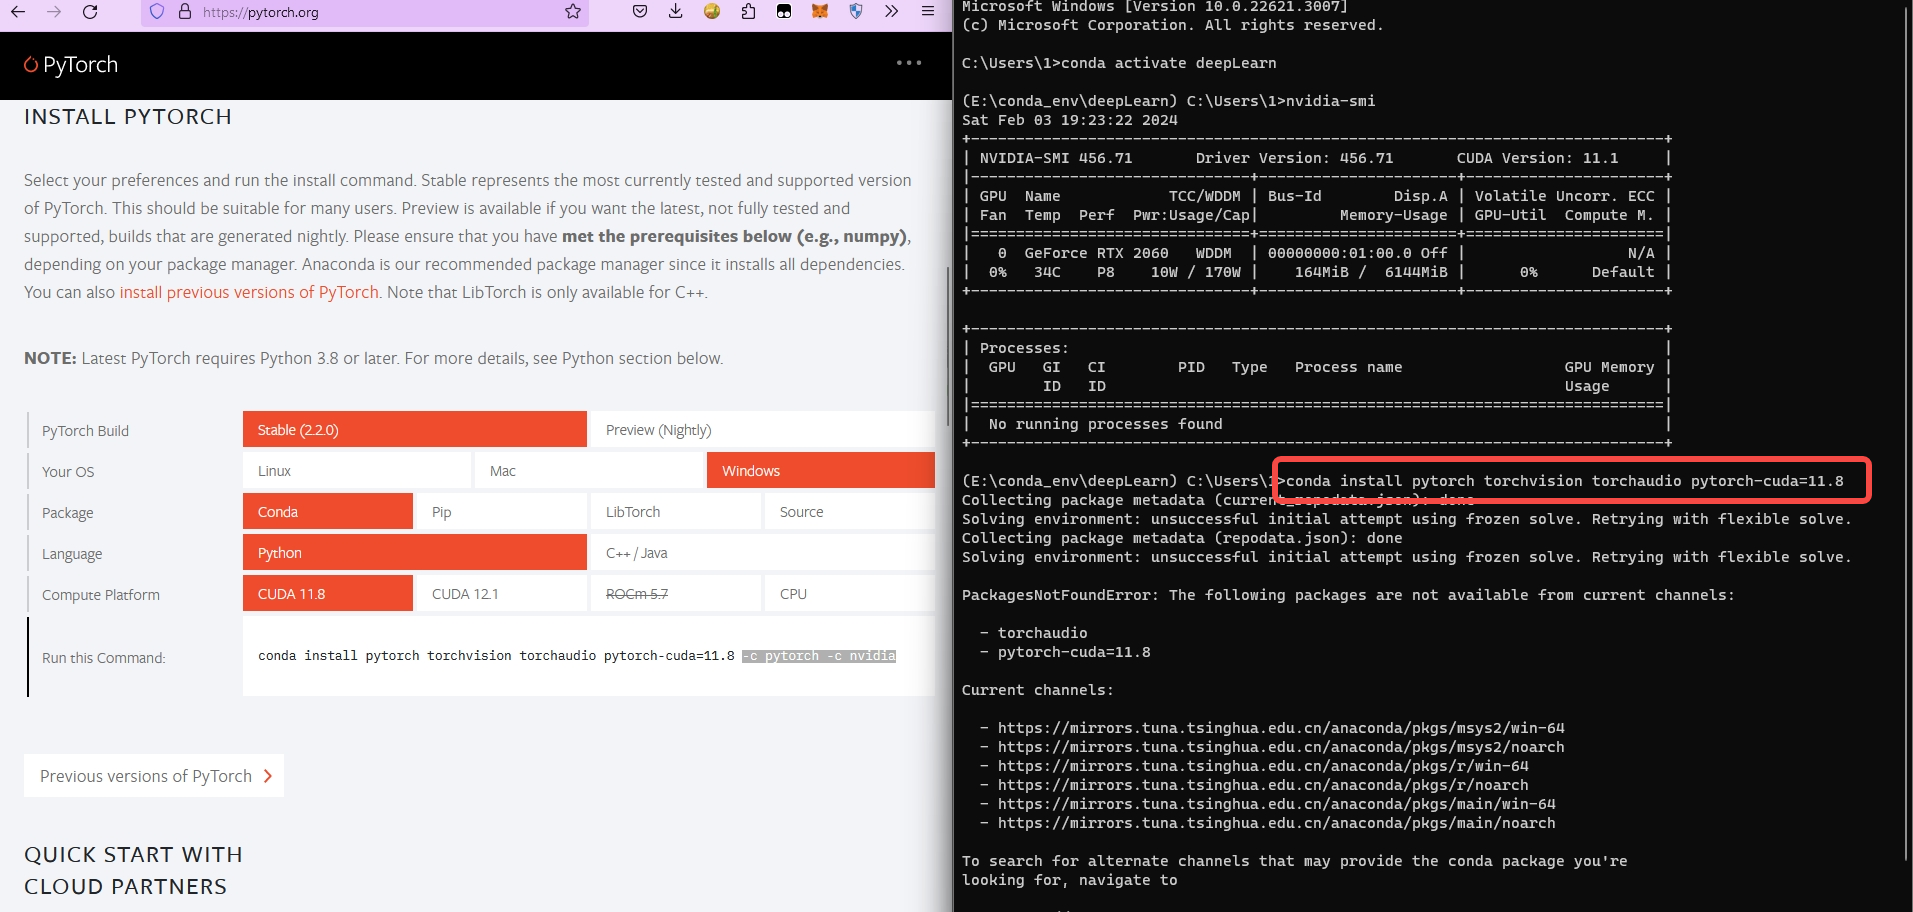
\includegraphics[width=.6\linewidth]{part/软件工程/环境搭建/虚拟环境/anaconda/pic/conda安装pytorch.png}
      \caption{\label{fig:conda安装pytorch}conda安装pytorch}
\end{figure}
\subsubsubsection{pip安装}
pip安装会比较快，但是相关依赖的包可能不会被安装
\begin{lstlisting}[style=demostyle,numbers=none]
pip3 install torch torchvision torchaudio --index-url https://download.pytorch.org/whl/cu118
\end{lstlisting}
\begin{figure}[htbp]
    \centering 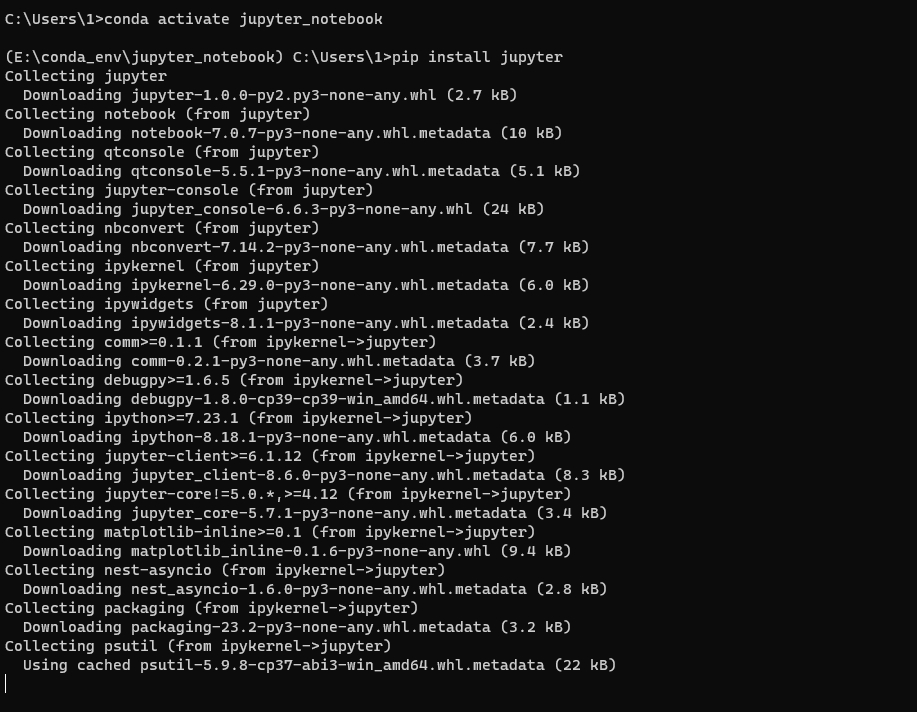
\includegraphics[width=.6\linewidth]{part/软件工程/环境搭建/虚拟环境/anaconda/pic/pip安装jupyter.png}
      \caption{\label{fig:pip安装jupyter}pip安装jupyter}
\end{figure}

\subsubsection{离线安装}
\label{subsubsec:install_package_offline}
如果有的包就一个可以到\href{https://pypi.org/}{pypi}上下载编译好的\codeinline{whl}文件，然后在命令行中输入
\begin{lstlisting}[style=demostyle,numbers=none]
pip install 包名
conda install 包名
\end{lstlisting}

\subsubsection{批量安装}
\label{subsubsec:install_package_batch}
事先写好一个\codeinline{requirements.txt}文件
\begin{lstlisting}[style=demostyle,numbers=none]
numpy
transformers==4.27.1
torch>=1.10
matplotlib
\end{lstlisting}    

然后在命令行中输入
\begin{lstlisting}[style=demostyle,numbers=none]
conda install --file requirements.txt
pip install -r requirements.txt
\end{lstlisting}

\subsection{卸载包}
\label{subsubsec:use_conda_package_remove}
\begin{lstlisting}[style=demostyle,numbers=none]
# 卸载包
conda remove <package_name>
conda uninstall <package_name>
\end{lstlisting}

\subsection{查看包}
\label{subsubsec:use_conda_package_list}
\begin{lstlisting}[style=demostyle,numbers=none]
# 查看所有已安装的包
conda list
# 查看指定环境下的包
conda list -n <env_name>
\end{lstlisting}

\subsection{更新包}
\label{subsubsec:use_conda_package_update}
\begin{lstlisting}[style=demostyle,numbers=none]
# 更新所有包
conda update --all

# 更新指定包
conda update <package_name>

## 更新conda本身
conda update conda
\end{lstlisting}

\subsection{清空缓存}
\label{subsubsec:use_conda_package_clean}
\begin{lstlisting}[style=demostyle,numbers=none]
# 清空缓存
conda clean --all
\end{lstlisting}

\section{Vscode配置}
\begin{figure}[htpb]
  \centering
  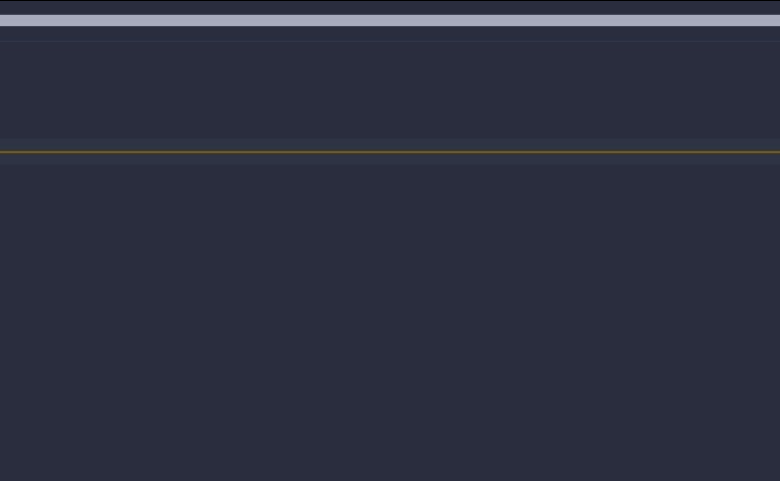
\includegraphics[width=0.6\textwidth]{part/软件工程/环境搭建/虚拟环境/anaconda/pic/vscode配置miniconda.png}
  \caption{修改python解释器}
  \label{fig:vscode配置miniconda-修改python解释器}
\end{figure}

\begin{figure}[htpb]
  \centering
  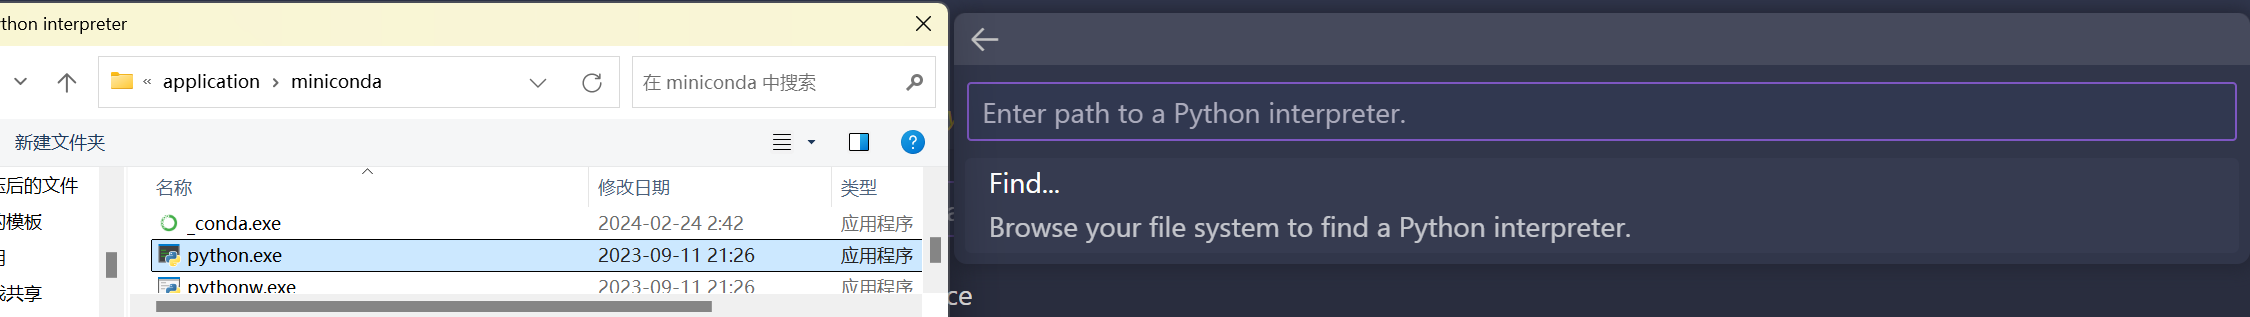
\includegraphics[width=0.6\textwidth]{part/软件工程/环境搭建/虚拟环境/anaconda/pic/选择conda的python解释器.png}
  \caption{选择conda的python解释器}
  \label{fig:选择conda的python解释器}
\end{figure}



